\documentclass[12pt]{article}
\usepackage[a4paper,margin=.5in]{geometry}
\usepackage{graphicx}
\usepackage{booktabs}
\usepackage{listings}
\usepackage{color}

\definecolor{dkgreen}{rgb}{0,0.6,0}
\definecolor{gray}{rgb}{0.5,0.5,0.5}
\definecolor{mauve}{rgb}{0.58,0,0.82}

\lstset{frame=tb,
  language=Python,
  aboveskip=3mm,
  belowskip=3mm,
  showstringspaces=false,
  columns=flexible,
  basicstyle={\small\ttfamily},
  numbers=none,
  numberstyle=\tiny\color{gray},
  keywordstyle=\color{blue},
  commentstyle=\color{dkgreen},
  stringstyle=\color{mauve},
  breaklines=true,
  breakatwhitespace=true,
  tabsize=3
}
%\usepackage{subfig}
\usepackage{subcaption}
\usepackage{hyperref}
\hypersetup{
    colorlinks=true,
    linkcolor=blue,
    filecolor=magenta,      
    urlcolor=cyan,
    pdftitle={Overleaf Example},
    pdfpagemode=FullScreen,
    }
\newcommand*{\figuretitle}[1]{%
    {\centering%   <--------  will only affect the title because of the grouping (by the
    \textbf{#1}%              braces before \centering and behind \medskip). If you remove
    \par\medskip}%            these braces the whole body of a {figure} env will be centered.
}
\title{Final Project}

\author{Tylman Michael\\CSE 546 Machine Learning}
%moderncv theme
\usepackage[utf8]{inputenc} 
\begin{document}
\maketitle{}
\section{Introduction}
Following from my progress report, I continued my iterative searches of optimal parameters, and aimed to cover the remaining 
requirements of this project. From my experiments, I decided to focus on using the following 4 classifiers: MLPNet, SVM, RF, 
and Naive Bayes (NB). From these 4 classifiers, I investigated different combinations of preprocessing with PCA or Cluster mapping, 
singular classifier ensemble methods like adaboost and bagging, and multiple classifier stacking.

I will explain the process of my experiments, but I will not go into large amounts of detail on the specific hyperparameters I attempted 
unless it is pertinent to the discussion because I performed a large amount of incremental experiments as I progressed on this project.

\section{Cluster Mapping}
After many iterations, I came to the conclusion that cluster mapping for this application is not useful, at least when used as a singular 
approach. Not one combination of pipeline steps I attempted were improved by cluster mapping for any classifier. I attempted PCA before and after mapping 
with several component options. I attempted utilizing them in adaboost and bagging. Nothing seemed to be improved by cluster mapping. Evidence of 
this can be seen in \ref{figure1} where I show examples of how kmeans mapping became a hinderance regardless of the hyperparameters it is coupled 
with. I do acknowledge that many of these items only show that I tried kmeans around or below 300 clusters, however I did attempt upwards of 
400 clusters in other experiments to have nearly identical results.

\begin{figure}
  \begin{subfigure}{.5\textwidth}
      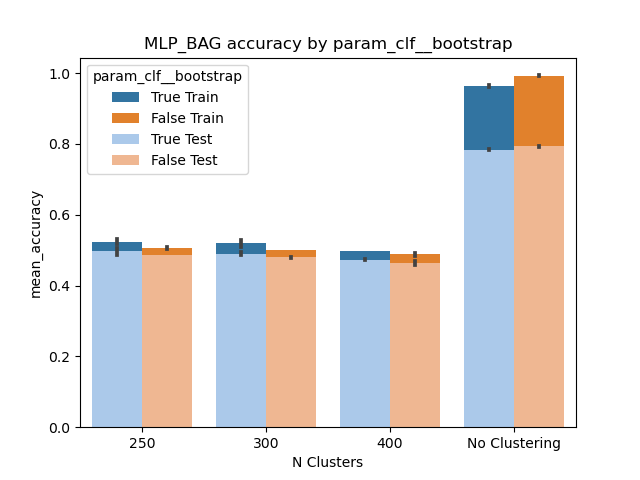
\includegraphics[width=.95\textwidth]{../../results_Exp6_kmeans_still_sucks/mlp_bag/param_clf__bootstrap_accuracy_param_Kmean.png}
      \caption{Bootstrapped MLP}
      \end{subfigure}%
    \begin{subfigure}{.5\textwidth}
      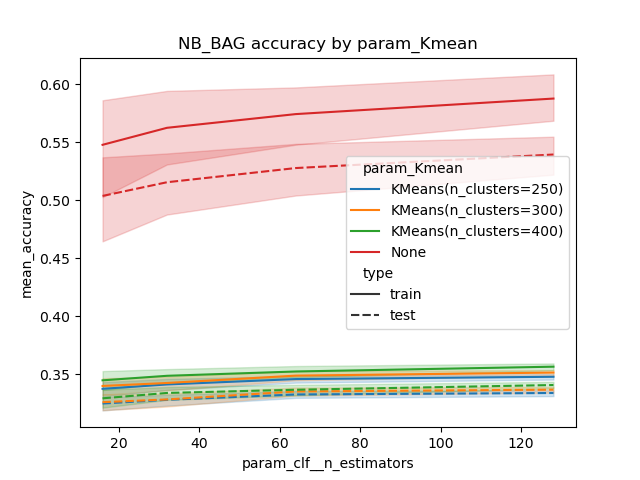
\includegraphics[width=.95\textwidth]{../../results_Exp6_kmeans_still_sucks/NB_bag/param_Kmean_accuracy_param_clf__n_estimators.png}
      \caption{Bagging NB}
    \end{subfigure}
    \begin{subfigure}{.5\textwidth}
      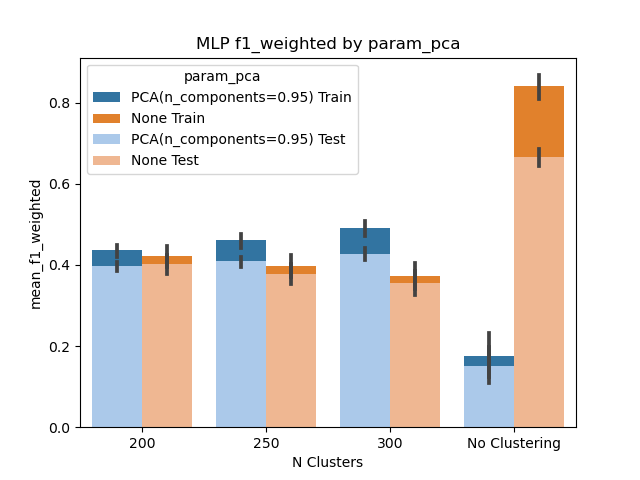
\includegraphics[width=.95\textwidth]{../../results_Experiment5_Final_No_Agg/mlp/param_pca_f1_weighted_param_Kmean.png}
      \caption{Singular MLP}
      \end{subfigure}%
    \begin{subfigure}{.5\textwidth}
      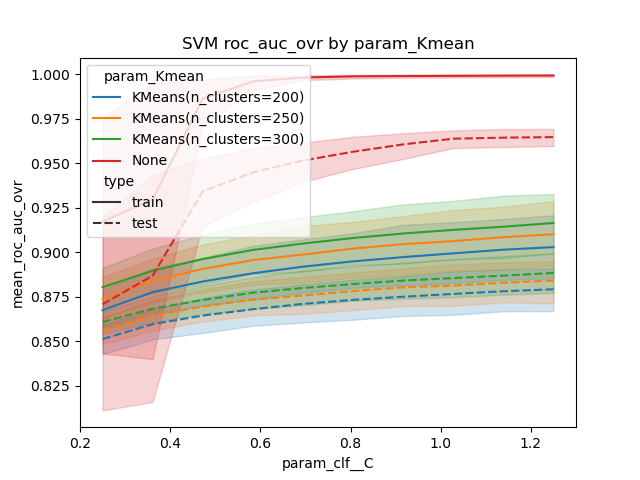
\includegraphics[width=.95\textwidth]{../../results_Experiment5_Final_No_Agg/svm/param_Kmean_roc_auc_ovr_param_clf__C.png}
      \caption{Singular SVM}
    \end{subfigure}
    \begin{subfigure}{.5\textwidth}
      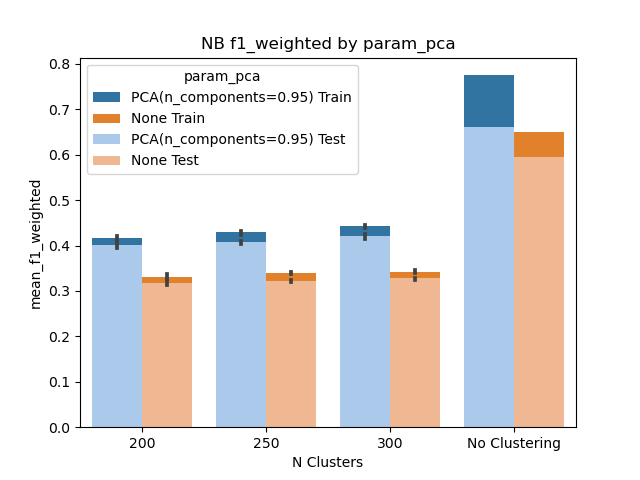
\includegraphics[width=.95\textwidth]{../../results_Experiment5_Final_No_Agg/nb/param_pca_f1_weighted_param_Kmean.png}
      \caption{Singular NB}
      \end{subfigure}%
    \begin{subfigure}{.5\textwidth}
      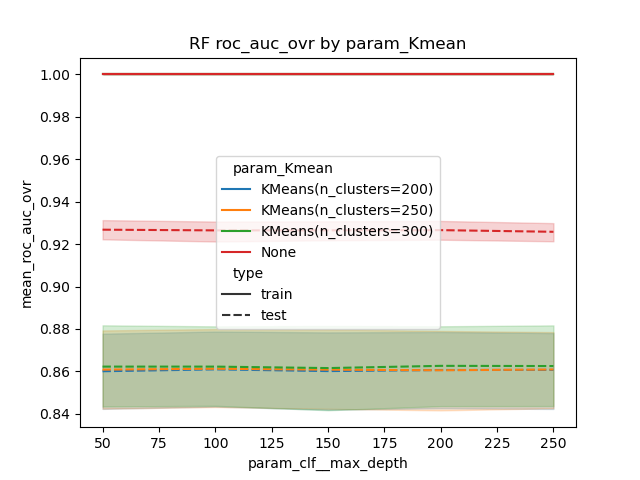
\includegraphics[width=.95\textwidth]{../../results_Experiment5_Final_No_Agg/rf/param_Kmean_roc_auc_ovr_param_clf__max_depth.png}
      \caption{Singular RF}
    \end{subfigure}
    \caption{KMeans Cluster Mapping Results}
    \label{figure1}
\end{figure}

Each of these experiments showed that cluster mapping was a hinderance, and that the original feature space was better. 
From these experiments, I decided to throw out the prospect of using Cluster Mapping as a preprocessing step for every method except the 
stacking ensemble method, which I will cover later.

\section{Ensemble Methods}
Before we are able to analyze how the models were effected by ensembling, we must take a moment to look at the performance of the best 
individual models so far compiled in Table \ref{table1}. I compiled the "winning" model for each of the four attempted classifiers showing 
their mean and standard deviation scores for train and validation splits across the metrics of accuracy, f1 score, and roc\_auc\_ovr. I 
additionally held out 20\% of my data as a test set to be tested once the model was finished and retrained on all data. 

I was planning to have a more in-depth discussion regarding the selection of the best hyperparameters for each of these models, but each of these models
showed such strong results when compared to their peers. Each of the models in this phase placed number 1 in all three mean validation score metrics, 
and showed either minimal reduction or improvement in performance when moving to the hold out test set. This improvement in performance for the test
set provided evidence to me that these high scores were not due to overfitting. If they were overfit, then providing more data would likely increase 
overfitting, which would show a decrease in testing scores. Since this is not the case, I will wait to show the in-depth performance analysis for only 
a couple models once we include the ensemble methods to save space.

Regardless, we can see that the MLPNet and the SVM classifiers are performing a cut above the Naive Bayes and Random Forest classifiers. This 
is a reasonable result since the feature space was generated by a CNN that was designed to optimize the performance of a network which likely 
had a least a portion of it representable by a standard MLP classifier. Likewise, historically Kernel SVM classifiers were known as the top 
performers in Machine Learning until the rise of deep networks, which is showing up again here. 

It is also reasonable that the Naive Bayes classifier will underperform because it requires some mathematical assumptions which a CNN is 
under no obligation to achieve for feature generation. The only thing surprising about this table is the behavior of the random forest 
classifier. It seems odd that it would be the only classifier to show a reduction in performance in the final testing phase. I am going to return 
to this question later on once we cover what happens to the other models when we perform ensembling.

Regardless, these results are very promising. They are almost too promising, in fact. My biggest concern from this point is overfitting, but 
that can actually lead to a benefit once we move on to ensembling. It's okay to have a diverse set of ensembles that are overfit on their own, 
as they may perform better together. 


\begin{table}
  \resizebox*{.95\textwidth}{!}{\begin{tabular}{lllllll}
\toprule
{} &                   stack &                  NBbag &                 mlpbag &                  NBada &                treeada &                  SVMbag \\
\midrule
Index                       &                       2 &                    867 &                     14 &                     51 &                     47 &                      17 \\
mean\_fit\_time               &      1405.5506918430328 &     40.285290360450745 &      579.3783206343651 &     102.77094876766205 &      1229.745915234089 &      129.07705068588257 \\
std\_fit\_time                &       56.74206058134601 &     0.6317175670817758 &      7.455601391413241 &     0.8867015999451987 &     1.8724155730382983 &       9.796660667519168 \\
mean\_score\_time             &      11.178422927856445 &      51.00288212299347 &     0.5981229543685913 &     48.676812052726746 &      3.830958664417267 &      27.196506679058075 \\
std\_score\_time              &       1.405742496910865 &     1.8923625091969507 &    0.11387845129075089 &     1.8198226356237728 &    0.28462153313195493 &       4.294021210732005 \\
mean\_test\_accuracy          &                    0.79 &     0.5754999999999999 &                0.79525 &                  0.637 &                0.54825 &                 0.77575 \\
std\_test\_accuracy           &   0.0022360679774997916 &   0.019868316486305507 &   0.008525696452489974 &    0.01383835250309806 &     0.0067961386095341 &     0.00831790237980707 \\
rank\_test\_accuracy          &                       5 &                     44 &                      1 &                      1 &                      1 &                       2 \\
mean\_train\_accuracy         &      0.9977499999999999 &                0.62925 &     0.9940833333333333 &     0.8125833333333333 &                  0.764 &                 0.99425 \\
std\_train\_accuracy          &   0.0007592027982620297 &   0.004872684635347887 &  0.0009537935951883014 &    0.01061281981588514 &    0.01018713785995741 &   0.0008620067027324092 \\
mean\_test\_f1\_weighted       &      0.7912570496724283 &     0.5858494831502836 &     0.7949238630429338 &     0.6431246854754509 &     0.5576218846400178 &      0.7762111731817483 \\
std\_test\_f1\_weighted        &   0.0029872474406088608 &    0.01903181076309097 &   0.008385994462715676 &   0.012909250517893546 &   0.007753848653095678 &    0.009018811244895598 \\
rank\_test\_f1\_weighted       &                       3 &                     38 &                      1 &                      1 &                      1 &                       2 \\
mean\_train\_f1\_weighted      &      0.9977507823245164 &     0.6389193533117794 &     0.9940841593977978 &     0.8137017737836371 &     0.7653651061845691 &      0.9942576816522287 \\
std\_train\_f1\_weighted       &   0.0007583764213535456 &   0.005289021391854054 &  0.0009541156349656866 &   0.010307792046297188 &   0.010124753277141824 &   0.0008584699193975221 \\
mean\_test\_roc\_auc\_ovr       &      0.9730999015536933 &     0.9088672548387857 &     0.9749867328830162 &     0.9364586653065938 &     0.8743949551758458 &      0.9688421608215558 \\
std\_test\_roc\_auc\_ovr        &    0.000915550433627727 &   0.006604637647041263 &  0.0008938521311151068 &  0.0030788513632281837 &  0.0034540071161737835 &   0.0019750940256677376 \\
rank\_test\_roc\_auc\_ovr       &                       1 &                      1 &                      1 &                      1 &                      1 &                       1 \\
mean\_train\_roc\_auc\_ovr      &      0.9999612015765678 &     0.9389531956927522 &     0.9999600333256833 &     0.9844012423207428 &      0.949929571828595 &       0.999923288362849 \\
std\_train\_roc\_auc\_ovr       &  2.4671281578632394e-05 &  0.0030594180625836366 &  1.558742578374733e-05 &  0.0010215200718514444 &   0.002438923495362692 &  3.1182187144615235e-05 \\
best\_final\_test\_accuracy    &                    0.96 &                  0.602 &                  0.961 &                   0.75 &                  0.714 &                   0.791 \\
best\_final\_test\_roc\_ovr     &      0.9989464604987599 &      0.927274695189538 &      0.996860066599987 &     0.9706142287135784 &     0.9326248076880352 &      0.9701864899787338 \\
best\_final\_test\_f1\_weighted &      0.9600616632865854 &     0.6136405868499072 &     0.9609942113384318 &      0.752537870834654 &     0.7160316970317154 &      0.7909626666332018 \\
\bottomrule
\end{tabular}
}
  \caption{Best Results and MetaData Singular}
  \label{table1}
\end{table}

\subsection{Bagging}
For the Bagging portion of my experiments, I took the best performing models of each type individually and re-trained them on 
the data using the same hyperparameters of the individual model. So, when I compare a bagged model vs. a standalone model, I am 
comparing the same model just trained differently.

I attempted to bag MLPnet, Naive Bayes, and the SVM classifiers. I did not attempt to bag the random forest classifier, since the 
random forest classifier is already a bagging style ensemble of decision trees. 

For MLPNet, we saw a moderate increase in performance across all metrics, pushing our final test accuracy up to be 95.6\%. This improvement 
is welcome, and the model selected was once again the best model for all metrics which shows strong consistency. I only did 16 classifiers
with 75\% of features and samples used 
for this bootstrapping due to the time constraints. Interestingly the model which performed the best is the model that bootstrapped the 
features and not the samples. 

In Figure \ref{figure2} we can see that bootstrapping samples (Where bootstrap True) provided a performance boost when we were applying 
cluster mapping, but when we did not use cluster mapping we saw performance drop if we bootstrapped the samples. But we can also see on the second row that 
the opposite held true for bootstrapping features. So, if we were mapping we wanted to reuse samples, but if we were not mapping we wanted 
to reuse features. I found this to be a fascinating turn of events that I haven't quite been able to fully explain yet. 

\begin{figure}
  \begin{subfigure}{.5\textwidth}
      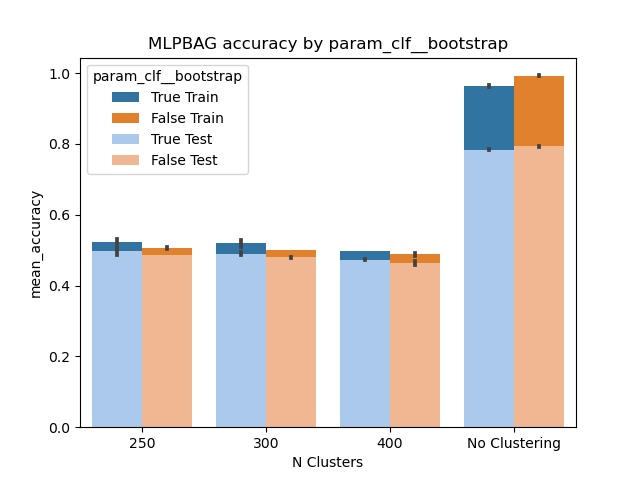
\includegraphics[width=.95\textwidth]{../../results/mlpbag/param_clf__bootstrap_accuracy_param_Kmean.png}
      \caption{Features Bootstrapping accuracy}
      \end{subfigure}%
    \begin{subfigure}{.5\textwidth}
      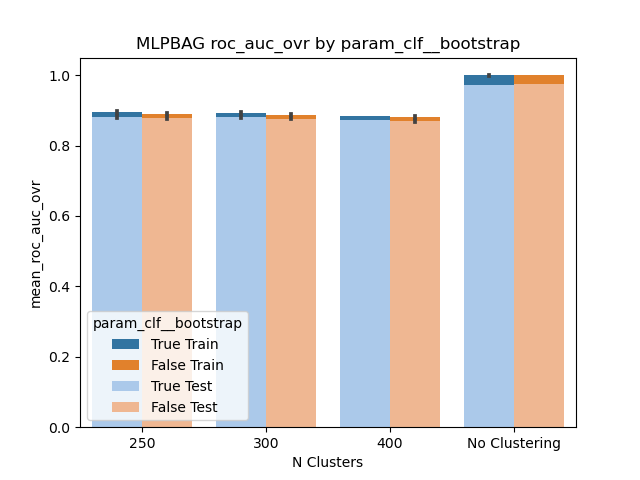
\includegraphics[width=.95\textwidth]{../../results/mlpbag/param_clf__bootstrap_roc_auc_ovr_param_Kmean.png}
      \caption{Samples Bootstrapping ROC}
    \end{subfigure}
    \begin{subfigure}{.5\textwidth}
      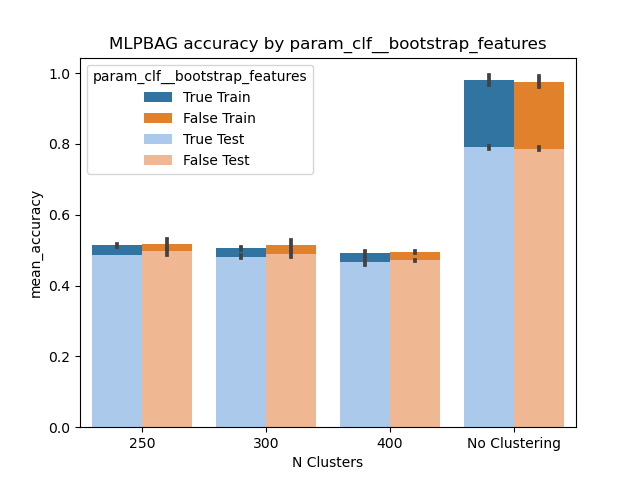
\includegraphics[width=.95\textwidth]{../../results/mlpbag/param_clf__bootstrap_features_accuracy_param_Kmean.png}
      \caption{Features Bootstrapping accuracy}
      \end{subfigure}%
    \begin{subfigure}{.5\textwidth}
      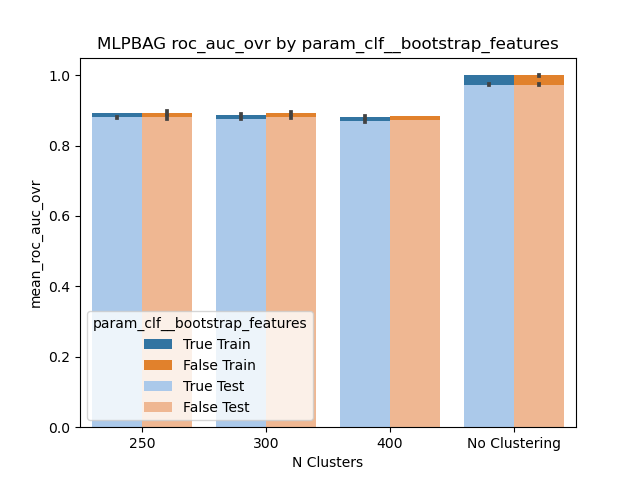
\includegraphics[width=.95\textwidth]{../../results/mlpbag/param_clf__bootstrap_features_roc_auc_ovr_param_Kmean.png}
      \caption{Features Bootstrapping ROC}
    \end{subfigure}
    \caption{MLPNet Bagging results}
    \label{figure2}
\end{figure}

\begin{table}
  \resizebox*{.95\textwidth}{!}{\begin{tabular}{lllllll}
\toprule
{} &                   stack &                  NBbag &                 mlpbag &                  NBada &                treeada &                  SVMbag \\
\midrule
Index                       &                       2 &                    867 &                     14 &                     51 &                     47 &                      17 \\
mean\_fit\_time               &      1405.5506918430328 &     40.285290360450745 &      579.3783206343651 &     102.77094876766205 &      1229.745915234089 &      129.07705068588257 \\
std\_fit\_time                &       56.74206058134601 &     0.6317175670817758 &      7.455601391413241 &     0.8867015999451987 &     1.8724155730382983 &       9.796660667519168 \\
mean\_score\_time             &      11.178422927856445 &      51.00288212299347 &     0.5981229543685913 &     48.676812052726746 &      3.830958664417267 &      27.196506679058075 \\
std\_score\_time              &       1.405742496910865 &     1.8923625091969507 &    0.11387845129075089 &     1.8198226356237728 &    0.28462153313195493 &       4.294021210732005 \\
mean\_test\_accuracy          &                    0.79 &     0.5754999999999999 &                0.79525 &                  0.637 &                0.54825 &                 0.77575 \\
std\_test\_accuracy           &   0.0022360679774997916 &   0.019868316486305507 &   0.008525696452489974 &    0.01383835250309806 &     0.0067961386095341 &     0.00831790237980707 \\
rank\_test\_accuracy          &                       5 &                     44 &                      1 &                      1 &                      1 &                       2 \\
mean\_train\_accuracy         &      0.9977499999999999 &                0.62925 &     0.9940833333333333 &     0.8125833333333333 &                  0.764 &                 0.99425 \\
std\_train\_accuracy          &   0.0007592027982620297 &   0.004872684635347887 &  0.0009537935951883014 &    0.01061281981588514 &    0.01018713785995741 &   0.0008620067027324092 \\
mean\_test\_f1\_weighted       &      0.7912570496724283 &     0.5858494831502836 &     0.7949238630429338 &     0.6431246854754509 &     0.5576218846400178 &      0.7762111731817483 \\
std\_test\_f1\_weighted        &   0.0029872474406088608 &    0.01903181076309097 &   0.008385994462715676 &   0.012909250517893546 &   0.007753848653095678 &    0.009018811244895598 \\
rank\_test\_f1\_weighted       &                       3 &                     38 &                      1 &                      1 &                      1 &                       2 \\
mean\_train\_f1\_weighted      &      0.9977507823245164 &     0.6389193533117794 &     0.9940841593977978 &     0.8137017737836371 &     0.7653651061845691 &      0.9942576816522287 \\
std\_train\_f1\_weighted       &   0.0007583764213535456 &   0.005289021391854054 &  0.0009541156349656866 &   0.010307792046297188 &   0.010124753277141824 &   0.0008584699193975221 \\
mean\_test\_roc\_auc\_ovr       &      0.9730999015536933 &     0.9088672548387857 &     0.9749867328830162 &     0.9364586653065938 &     0.8743949551758458 &      0.9688421608215558 \\
std\_test\_roc\_auc\_ovr        &    0.000915550433627727 &   0.006604637647041263 &  0.0008938521311151068 &  0.0030788513632281837 &  0.0034540071161737835 &   0.0019750940256677376 \\
rank\_test\_roc\_auc\_ovr       &                       1 &                      1 &                      1 &                      1 &                      1 &                       1 \\
mean\_train\_roc\_auc\_ovr      &      0.9999612015765678 &     0.9389531956927522 &     0.9999600333256833 &     0.9844012423207428 &      0.949929571828595 &       0.999923288362849 \\
std\_train\_roc\_auc\_ovr       &  2.4671281578632394e-05 &  0.0030594180625836366 &  1.558742578374733e-05 &  0.0010215200718514444 &   0.002438923495362692 &  3.1182187144615235e-05 \\
best\_final\_test\_accuracy    &                    0.96 &                  0.602 &                  0.961 &                   0.75 &                  0.714 &                   0.791 \\
best\_final\_test\_roc\_ovr     &      0.9989464604987599 &      0.927274695189538 &      0.996860066599987 &     0.9706142287135784 &     0.9326248076880352 &      0.9701864899787338 \\
best\_final\_test\_f1\_weighted &      0.9600616632865854 &     0.6136405868499072 &     0.9609942113384318 &      0.752537870834654 &     0.7160316970317154 &      0.7909626666332018 \\
\bottomrule
\end{tabular}
}
  \caption{Best Results and MetaData Ensemble}
  \label{table2}
\end{table}


For the Naive Bayes Classifier, bagging proved to be a terrible choice. The stability of the different performance metrics broke down, showing 
that this model was not classifying classes with nearly an consistency. The model shown is the model which gave the best ROC score, but it placed 
44th in Accuracy score and it placed 38th in Weighted F1 score. Additionally, all of these scores have decreased! So bagging the Naive Bayes model
completely broke down its already poor efficacy, and removed the only strength it had which was consistency. Naive Bayes is continuing to show that 
it is not the model appropriate for this data, which is what I expected coming in to this portion.

For the SVM Classifier, bagging appeared to lower it's overall effectiveness, but it became very stable when moving to testing. The mean validation 
scores behaved very closely to the holdout set scores. Additionally, the cross-validation results were remarkably stable. Showing little difference 
in overall performance as we change the percentage of samples or features used, as shown in \ref{figure3}.
If I were to choose to employ the orignal SVM or this bagged SVM classifier, I'd more likely go for the bagged SVM classifier because I trust it's 
generalizability more than a single SVM. 

\begin{figure}
  \begin{subfigure}{.5\textwidth}
      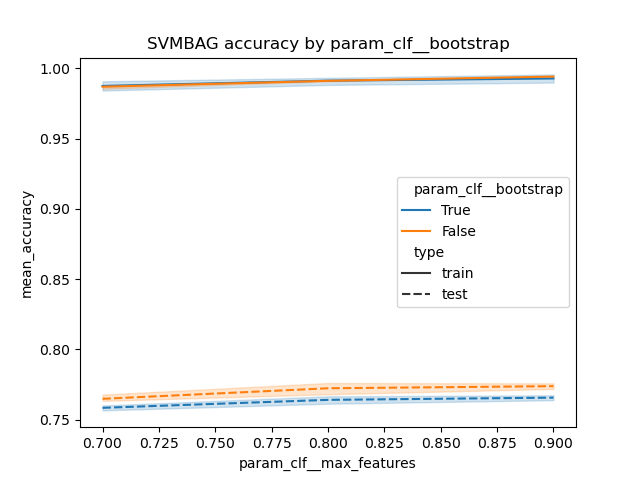
\includegraphics[width=.95\textwidth]{../../results/SVMbag/param_clf__bootstrap_accuracy_param_clf__max_features.png}
      \caption{Max Features Accuracy}
      \end{subfigure}%
    \begin{subfigure}{.5\textwidth}
      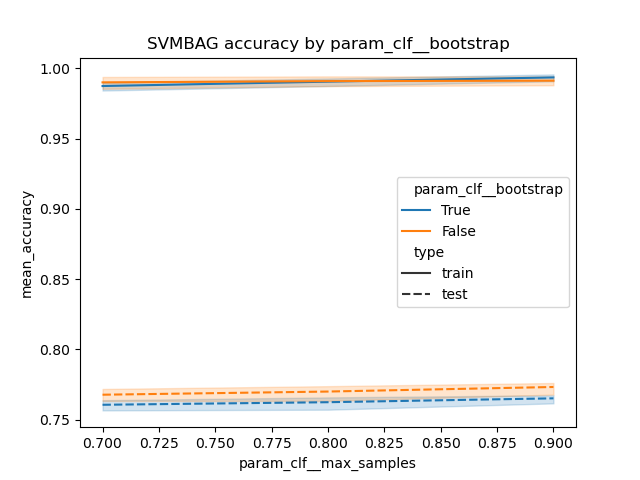
\includegraphics[width=.95\textwidth]{../../results/SVMbag/param_clf__bootstrap_accuracy_param_clf__max_samples.png}
      \caption{Max Samples Accuracy}
    \end{subfigure}
    \begin{subfigure}{.5\textwidth}
      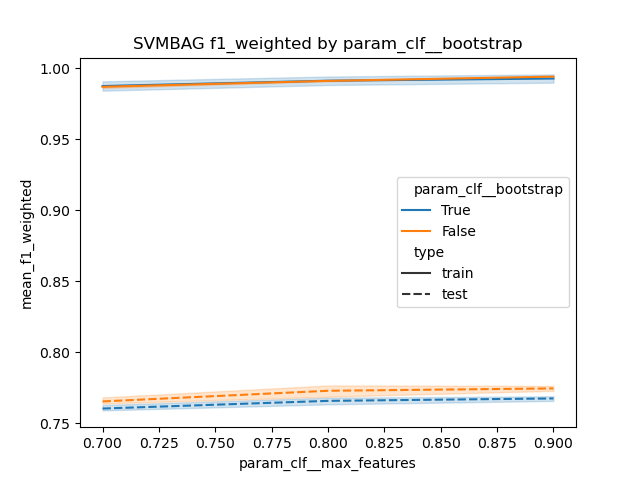
\includegraphics[width=.95\textwidth]{../../results/SVMbag/param_clf__bootstrap_f1_weighted_param_clf__max_features.png}
      \caption{Max Features Weighted F1}
      \end{subfigure}%
    \begin{subfigure}{.5\textwidth}
      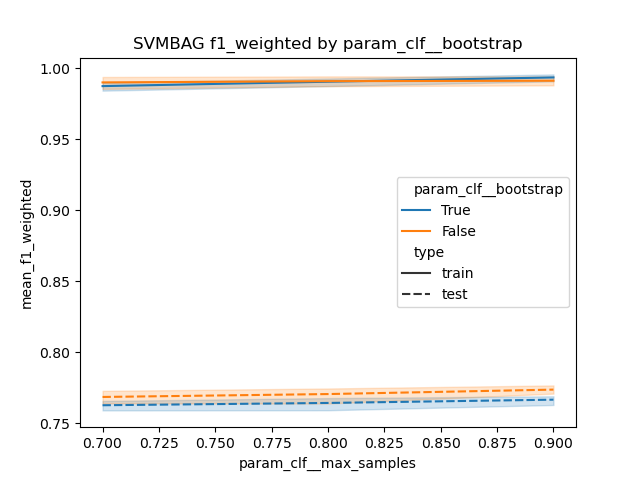
\includegraphics[width=.95\textwidth]{../../results/SVMbag/param_clf__bootstrap_f1_weighted_param_clf__max_samples.png}
      \caption{Max Samples Weighted F1}
    \end{subfigure}
    \begin{subfigure}{.5\textwidth}
      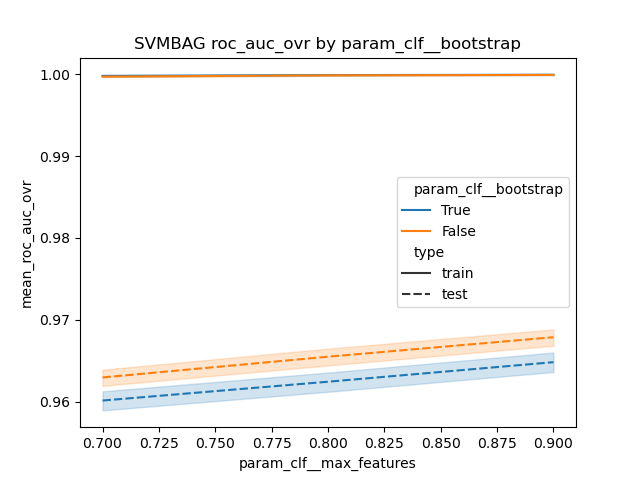
\includegraphics[width=.95\textwidth]{../../results/SVMbag/param_clf__bootstrap_roc_auc_ovr_param_clf__max_features.png}
      \caption{Max Features ROC AUC}
      \end{subfigure}%
    \begin{subfigure}{.5\textwidth}
      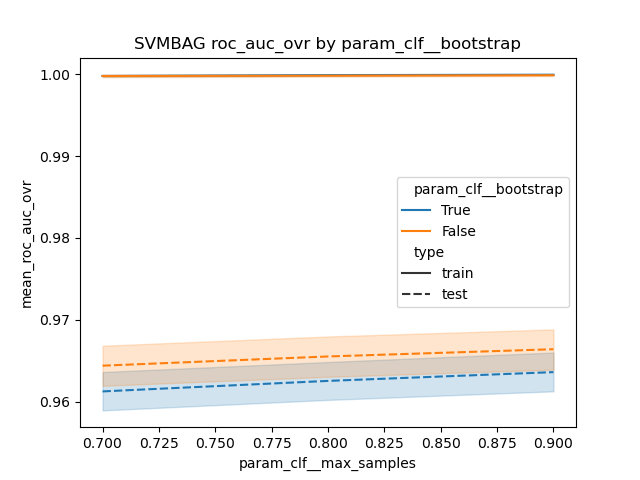
\includegraphics[width=.95\textwidth]{../../results/SVMbag/param_clf__bootstrap_roc_auc_ovr_param_clf__max_samples.png}
      \caption{Max Samples ROC AUC}
    \end{subfigure}
    \caption{SVM Bagging results}
    \label{figure3}
\end{figure}

\subsection{AdaBoost}
I only attempted to adaboost the Naive Bayes classifier, and a basic decision tree classifier because of Adaboost's requirement of a "weak" 
learner. I also did not have much faith in boosting for this project, since my base non-weak classifiers were performing so well. However, I 
gave it a shot to meet the criteria for the assignment and maybe challenge my pre-conceived notions.

Luckily, boosting fixed the consistency issue for Naive Bayes so all criteria are back to being scored at number 1 for the winning model. 
Boosting also improved performance over bagging for all metrics, but it appears to have done more overfitting. The training scores and the 
validation scores were previously extremely close to one another, but now there's a definite improvement to training scores that is more pronounced
than the improvement to the test scores. These results push the training scores for all metrics above the standalone NB classifier's training
means, but the boosted classifier is getting worse validation and test results.

The Boosted Decision Tree classifier performed better than I expected on this data. It is able to outperform the random forest classifier, and 
the bagged Naive Bayes classifier. However, it is unable to keep pace with the current front runners on any metric, and it comes at an 
extremely steep training cost nearly doubling the amount of time it took to train a bootstraped MLPNet of 16 models. I knew boosting had a 
tendency to take longer than other methods, but I did not expect it to take this long. After I received my first results with this model and 
saw it's mediocre performance at a cost of the largest training time observed yet, I immediately pulled the plug on attempting to employ it any 
longer. 

Overall, I was so unimpressed by AdaBoost on this dataset that I would have excluded the experiments investigating it alongside the many other 
experiments I attempted that didn't make the cut to be included in this report. However, since it was a base requirement of the project to 
use Adaboost, I included the results in my tables for a couple models to show that I did attempt Adaboost.

\subsection{Stacking}
Now onto the grand finale of all of this work: Model Stacking. To find the best model stacking combination, I first threw out the Naive Bayes 
classifier because it was lacking in performance. Sure, it's answers were uncorrelated with the other classifiers, but in my preliminary tests
all of the best model combinations avoided the Naive Bayes classifier like the plague. It was necessary to remove one of the classifiers in order 
for me to be able to enact my plan in a timely manner.

My plan was to investigate the value of utilizing kmeans mapping as a way of decorrelating our classifiers that are now forced to use different 
features. The way I planned on doing this was to create a set of pipelines where the best MLPNet, SVM, and RF model were taken and placed as 
the classifier in new pipelines which contained either a Kmeans mapping and a PCA step, or just a PCA step. The PCA step for both of these options
is very minimal, keeping 99\% of the variance and is only intended on forcing orthogonal features and removing only the most redundant dimensions.

Once I had this list of 6 pipelines, I then created a master list of all possible combinations of 4 out of the 6 of them. I then added on 
3 more sets to this list. One is made up of only plain pipelines, one is made up of only KMeans pipelines, and one is made up of all 6. I chose 
this approach because I was attempting to show that there is a benefit to using different projections of data to create diversity, and by having 
3 plain combined with 3 mapped pipelines, I could guarantee that we get at least one model different from the others. By including additional 
combinations that use all 6 options and only options which share the same input data, we can see if there's any benefit we are gaining 
that is greater than either A: the inherit benefit of using as many classifiers as possible or B: the benefit of using different classifiers
regardless of their input space. Finally, I used both a Linear SVM and a Logistic Regressor for the final estimator on top of all else.

I will show the top scoring model across all 3 metrics, alongside the 3 special test models in Table \ref{table3}. We can right away see 
that the F1 score and accuracy scores prefer to use the Calibrated SVM, while the ROC curve favored the Linear Regressor. Interestingly,
by sheer luck the top 3 scoring F1 scores are all represented here, and we can se how tightly stacked the accuracies are with only a very small 
margin between them. Each of the top scoring models for their respective metric are placing high in all of the other metrics except for the top 
ROC model. That model is placed only 19th and 16th out of 34 models for accuracy and F1 score. Why is this? 

Well, the Calibrated SVM produces it's probability predictions by doing an internal calibration, whereas the logistic regressor comes out of the 
box with probability outcomes. This leaves the SVM to have some more instability in it's probability scores, which will lead to inconsistencies that 
causes models which use this final step to be less likely to give a good roc score. 

Given how well this model is performing, and how robust to overfitting it likely 
is due to the nature of stacked models, I plan on comparing the stacked model for my final analysis and testing.
The sub model that I plan on using is the maximized accuracy model, since this assingment 
is listed as being tested on accuracy on the provided test set, and the top models of this type being so closely stacked anyway.

\begin{table}
  \resizebox*{.95\textwidth}{!}{\begin{tabular}{llrrrrrr}
\toprule
   param\_final\_estimator &                                               name &  mean\_test\_accuracy &  rank\_test\_accuracy &  mean\_test\_f1\_weighted &  rank\_test\_f1\_weighted &  mean\_test\_roc\_auc\_ovr &  rank\_test\_roc\_auc\_ovr \\
\midrule
    LogisticRegression() &        [Kmean\_mlp, Kmean\_svm, Kmean\_rf, plain\_svm] &             0.79000 &                   5 &               0.791257 &                      3 &               0.973100 &                      1 \\
CalibratedClassifierCV() &        [Kmean\_mlp, Kmean\_rf, plain\_mlp, plain\_svm] &             0.79100 &                   2 &               0.792747 &                      1 &               0.968521 &                     19 \\
CalibratedClassifierCV() &        [Kmean\_mlp, plain\_mlp, plain\_svm, plain\_rf] &             0.79150 &                   1 &               0.791693 &                      2 &               0.969073 &                     16 \\
    LogisticRegression() & [Kmean\_mlp, Kmean\_svm, Kmean\_rf, plain\_mlp, pla... &             0.78675 &                  13 &               0.788132 &                     11 &               0.972216 &                      4 \\
    LogisticRegression() &                   [Kmean\_mlp, Kmean\_svm, Kmean\_rf] &             0.69950 &                  29 &               0.700241 &                     29 &               0.946772 &                     30 \\
    LogisticRegression() &                   [plain\_mlp, plain\_svm, plain\_rf] &             0.78400 &                  21 &               0.784578 &                     22 &               0.968100 &                     21 \\
\bottomrule
\end{tabular}
}
  \caption{Stacked Model Interesting Results}
  \label{table3}
\end{table}

\section{Final analysis}
As I moved my final model over to a new file for the final analysis and to place it in a form fitting the deliverable 
requirements, I discovered an error in my generation of test data. Once I remedied that, my testing more closely 
coincided with what was being seen in cross-validation. This casts doubt on my previous results of accuracies in 
the mid 90s, but the experiments which led to those results took many overnight runs which I no longer have the time 
to revisit. The validation performance alone is good enough that when combined with our knowledge of meta-classifiers 
we can still justify using this stacked method for our final model. Regardless, the new performance metrics on 
the 20\% test set were an accuracy of 81\%, an ROC\_AUC of 97.26\%, and a weighted F1 score of 81.097\%.

Also once I fixed this bug, I discovered that the plain MLPNet classifier could not converge given the learning rate provided, 
so I allowed it to become an adaptive learning rate, which fixed the issue. With these newbie mistakes corrected, it's 
time to see how well the final model will really perform.



The first thing I tested was to find out when the stacking was helpful, and when the stacking was hurtful. 
So, I aggregated the outputs of each of the sub-models, and I gathered every time that 3 or 4 of the individual models 
guessed correctly but the stacked model guessed incorrectly. Out of a thousand samples, I found 3 cases where this 
occurred. I also looked for how often the combined model was better than the sum of its parts. I looked for 
all cases where only 1 or no models guessed correctly individually, but combined the stacked model was correct. I found
85 such samples. Given how large the number of samples which had 1 submodel correct was, I then looked for samples in which 
no models were correct individually. I found 2 such samples and plotted them in alongside the 
samples which were worse than their individual parts in Figure \ref{figure5}. 
\begin{figure}

    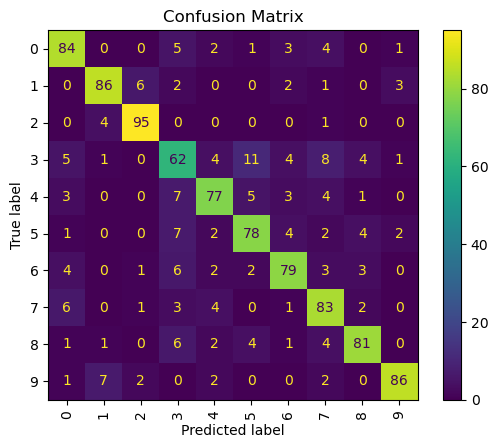
\includegraphics[width=.95\textwidth]{../../Deliverable/Final_CM.png}
    \caption{Confusion Matrix}
    \label{figure4}
\end{figure}


\begin{figure}
  \begin{subfigure}{.5\textwidth}
    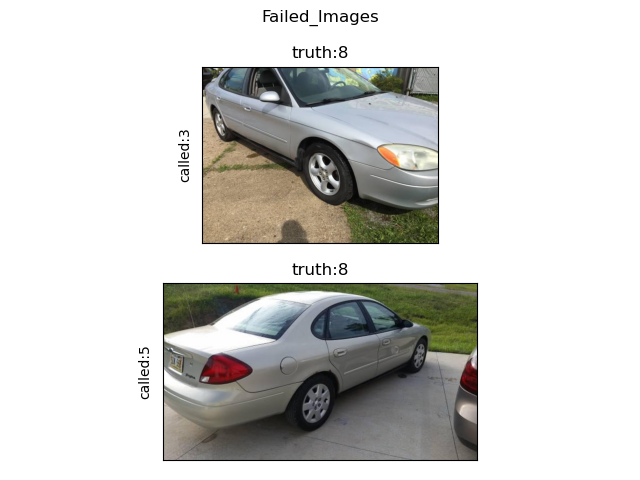
\includegraphics[width=.95\textwidth]{../../Deliverable/Failed_Images.png}
      \caption{Images Where Stacking Was Hurtful}
      \end{subfigure}%
    \begin{subfigure}{.5\textwidth}
      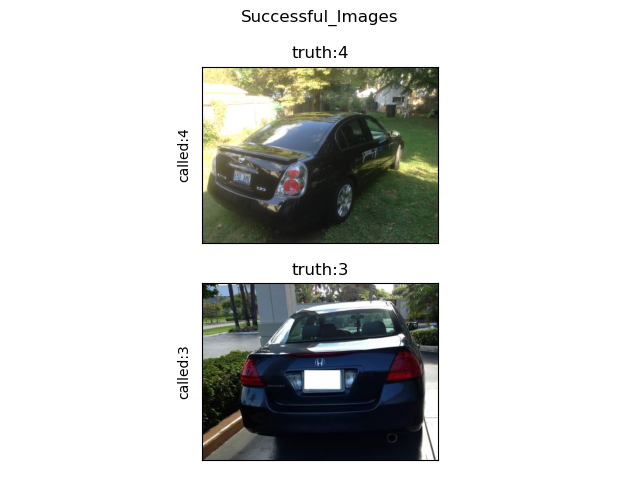
\includegraphics[width=.95\textwidth]{../../Deliverable/Successful_Images.png}
      \caption{Images Where Stacking Carried}
    \end{subfigure}

    \caption{Example Images Comparison}
    \label{figure5}
\end{figure}

% \begin{figure}
%   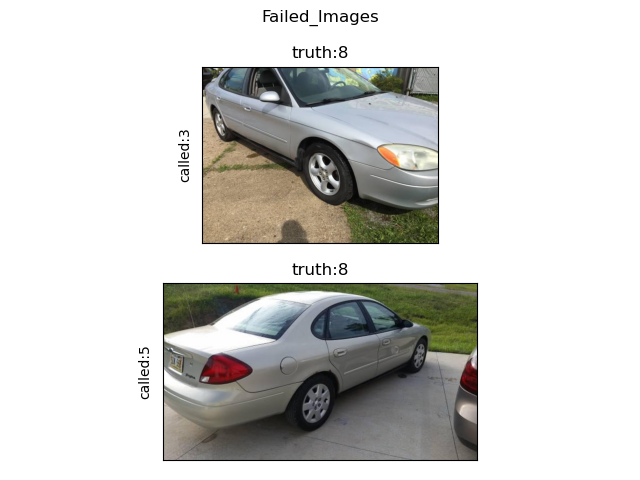
\includegraphics[width=.95\textwidth]{../../Deliverable/Failed_Images.png}
%   \caption{Images Where Stacking Was Hurtful}
%   \label{figure5}
% \end{figure}



% I also looked at the maximum value called for each of these images in 
% Table \ref{table4}. From this we can see all of them show moderate to low confidence for most of these results, especially the 
% random forest. Given the fact that there are only 5 samples out of 1000 test samples which show this behavior, and 
% the majority of them do not have high confidence I think we can conclude that this behavior is merely the result of chance on 
% low-confidence samples.
\begin{table}
  \resizebox*{.95\textwidth}{!}{\begin{tabular}{rrrr}
\toprule
 Kmean\_mlp\_max &  plain\_mlp\_max &  SVM\_max &   RF\_max \\
\midrule
      0.294212 &       0.537351 & 0.480996 & 0.166667 \\
      0.322180 &       0.389319 & 0.341622 & 0.191111 \\
      0.433741 &       0.738816 & 0.634804 & 0.126667 \\
\bottomrule
\end{tabular}
}
  \caption{Maximum Value For Each SubModel}
  \label{table4}
\end{table}

% Moving on from this revelation, 

% \begin{figure}
%   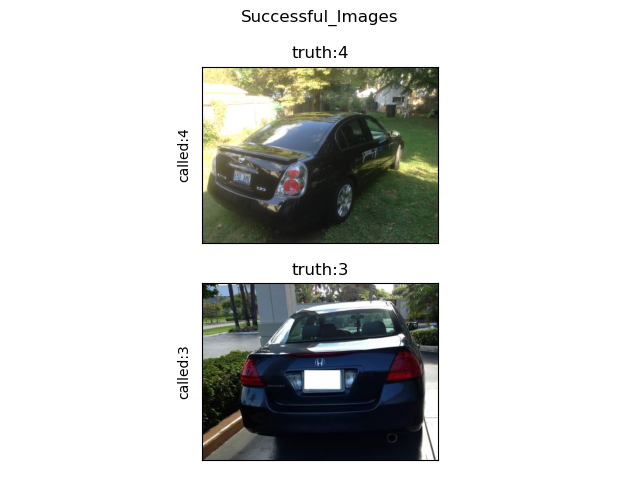
\includegraphics[width=.95\textwidth]{../../Deliverable/Successful_Images.png}
%   \caption{Images Where Stacking Carried}
%   \label{figure6}
% \end{figure}



The first image of the two which performed worse is a picture where a large portion of the car's outline is 
cut off. The only defining features present are the shape of the wheelwell, one headlight, and the shape of 
the rearview mirror. I'd be surprised if any models gave a high score to this sample. So, I included the individual 
submodel performances in Table \ref{table4}. Looking at this table, we can see that only one model had a confidence 
over .5, which would lead me to conclude that this is a low-confidence sample for all models involved.

The second image of the two which performed worse is not only also cut off, but it appears to have another 
car's tail light in the image which can easily confuse the classifiers. Additionally, its individual confidences 
were very low, with the highest called confidence being a .38. Looking at these images and confidences, we can conclude 
that these are just low confidence samples that got unlucky due to being cutoff. 

The first image of the two which were correct despite not having a single correct sub-model call is an image which 
has a very bright region dominating the top left. In my experiments (including those not mentioned), I've found that 
the individual models can struggle with images that have very bright white regions, likely due to how that can 
effect normalization. 

The second image has an area of the image censored by a pure white rectangle. This pure white rectangle could also 
cause similar issues to the blown out area of the first image, especially since it's located dead center in the
most important part of the image. Overall, the stacking classifier is capable of overcoming images where 
the individual classifiers may not be able to process due to the effect of singular bright area.


Looking at the confusion matrix, we can see that our very worst perfoming class is the Honda Accord, which is showing 
remarkably low performance compared to even the second-best model. Attempting to make sense of this, I manually browsed 
through the photos for each of these two classes, and I discovered that the Honda Accord has a wide variety of possible 
trunk configurations. Clicking through, I found several which had different forms of spoilers, tail lights, and exhaust 
pipes. I will show some examples of the variety in figure \ref{figure6}.

\begin{figure}
  \begin{subfigure}{.5\textwidth}
    \includegraphics[width=.95\textwidth]{../../Data/train_images/honda_accord_2005-2006/00000_4oxWGTcv0fR_600x450.jpg}
      \caption{Tall Spoiler, Disconnected Tail Lights, 1 Pipe}
      \end{subfigure}%
    \begin{subfigure}{.5\textwidth}
      \includegraphics[width=.95\textwidth]{../../Data/train_images/honda_accord_2005-2006/00d0d_YgO9qFF8W5_600x450.jpg}
      \caption{Tall Spoiler, Trio Tail Lights, 2 Pipes}
    \end{subfigure}
    \begin{subfigure}{.5\textwidth}
    \includegraphics[width=.95\textwidth]{../../Data/train_images/honda_accord_2005-2006/00B0B_6by35oNSQi9_600x450.jpg}
      \caption{No Spoiler, Trio Tail Lights, 1 Pipe}
    \end{subfigure}%
    \begin{subfigure}{.5\textwidth}
      \includegraphics[width=.95\textwidth]{../../Data/train_images/honda_accord_2005-2006/00E0E_84LfhT8owLo_600x450.jpg}
      \caption{No Spoiler, Connected Tail Lights, 0 Pipe}
    \end{subfigure}

    \caption{Example Images Comparison}
    \label{figure6}
\end{figure}

From these images we can see that the Honda Accord is a highly varied vehicle. I looked on Honda's website, and I found 
that the honda accord has 7 trim levels and 9 configurations to pick from, and the Honda Accord was ranked number one 
in popularity in America in 2022. Admittedly this does not specifically include 2005-2006 Honda Accords, but I think it's 
important to note that the Honda Accord is unusual in it's wide application. Additionally, the spoiler with split tail lights
configuration of the Honda Accord is very reminiscent of the rear end of a Ford Mustang, and the spoilerless configuration with
split tail lights is similar to a Toyota camry. I think the reason why the Honda Accord is performing so poorly is largely 
due to the fact that it is the small-profile car which may have connected and disconnected tail lights, so images taken 
from behind are at a severe disadvantage.

Overall, this model appears to be working well, and seems to be sound in design. The stacked method is perfoming better 
than the sum of its parts, and performing at a level that falls in the expected range of performance for a non-deep net method
as we had discussed in class. 

\end{document}